\section{Software Testing Life-cycle and Methodologies:}

\subsection{Software Testing and Test / Bug / Defect TAXONOMY}

Taxonomy means ORGANIZATIONAL SCHEMA

You must be disciplined in your thinking, and develop a strong mental model, an organizational SCHEMA, to describe and categorize Features and Defects(BUGS).

What are the CATEGORIES OF BUGS and occur in Applications?

Classifiers: Classifiers are terms that we use to put things in BUCKETS.
Designators: Are the names we call things by. In terms of software testing: Our DESIGNATORS are terms that make up to describe common patterns of software failure.

In general there are 3 kinds of Software Applications: (We need to ensure that we are familiar with the Methodologies to test each of these kinds of systems):

mobile, web and desktop
Integrated Software
Application, programming, system
system software,application software
System , application  , web app software
streaming, service provider & services consumer platform, social media

Embedded Systems/Application Programming : Raspberry PI, Ardunio, usually programmed in C (light, small foot print, because we have a lower powered CPU, small memory, low power consumption

Desktop / Server: C#, Java

Cloud based: AWS, Azure, Machine Learning, Language Translation / cloud based APIs, restful services

\section{There are 3 categories of Software Testing: }
\subsection{Unit Testing: At the Method Level}
To be a good candidate for Unit Testing, a method must be written in a very clear and unambiguous way.
The method should implement a well defined STATE TABLE: Meaning:

Note: Recall that a method has a METHOD SIGNATURE: visibility MethodName(method signature)
where the method signature is the set of input parameters to the methods: data type Name of parameter
and the method has a RETURN TYPE

\subsection{Our tool to do Unit Testing at the Method level is the STATE TABLE}
You will add a STATE TABLE to the work you did in your Learning Activity ONE - meaning, you will think about how to construct TEST RULES for your Methods.
You are going to make a Table (we will use EXCEL), and you are going to think for your METHODS: What OUTPUT SHOULD BE presented by the METHOD for various different possible sets of input conditions.

So the STATE TABLE is a table that states for different sets of input parameters, we expect specified return.

You use the State Table to define the TEST RULES.

The purpose of the Traceability Matrix is to connect/join the Behavior of each Method to the Requirement which that method should be servicing/implementing.

\subsection{Integration Testing: We test for the proper integration between method:}

The big tool we use to do Integration Testing is the Object Interaction Diagram.
You may wish to consider, to get hired as a Programmer, to the OMG (Object Management Group) UML Certification Exam.
\url{https://www.omg.org/uml-certification/Advanced.htm}

There are 5 kinds of UML Diagrams
You can see a reference here:
https://www.smartdraw.com/uml-diagram/#:~:text=%20Types%20of%20UML%20Diagrams%20%201%20Class,Composite%20structure%20diagram%206%20Deployment%20diagram%20More%20}

The main kinds of UML Diagrams that help us to understand our Software Application to write effective tests are:

Class Interaction Diagram
Object Interaction Diagram
Method Interaction diagram to visual the METHOD CHOREOGRAPHY

The goal here is to create effective, meaningful, comprehensive TEST RULES to use in creating our TEST CASES

If you can test your PRODUCT to a perfectly complete degree, you can write comprehensive and complete TEST CASES and not have any surprises or unexpected occurrences!

A great benefit of writing your code to be TESTABLE is you are now writing very good quality code:
Easy to support
Easy to maintain
Easy to document

\newpage

A Software Testing Lifecycle

Testing is the process of executing a software product on sample input data and analyzing its output. Unlike other engineering products, which are usually fault-free, software products are prone to be faulty, due to an accumulation of faults in all the phases of their lifecycle (faulty specifications, faulty design, faulty implementation, etc.). Also, unlike other engineering products, where faults arise as a result of product wear and/or decay, the faults that arise in software products are design faults, which are delivered with the new product.

3.1 A SOFTWARE ENGINEERING LIFECYCLE
The simplest model of a software product lifecycle views the process of developing and evolving the product as a set of phases proceeding sequentially from a requirements analysis phase to a product operation and maintenance phase. 

The product development lifecycle is what we get by the Unified Process Development Methodology.

Feasibility Analysis: Feasibility analysis is the phase when the economic and technical feasibility of the development project is assessed, and a determination is made of whether to proceed with the development project, within a given budget, schedule, and technological means.
Requirements Analysis: The phase of requirements analysis is the most difficult of the software lifecycle, at the same time as it is the most fateful phase, in terms of determining the fate of the project (its success or failure, its scope, its cost, its value to users, etc.). Whereas a naïve view may understand this phase as consisting of a user dictating user requirements and a software engineer who is carefully taking notes, the reality of this phase is typically much more complex: The requirements engineer (a software engineering specializing in analyzing requirements) must conduct a vast data gathering operation that consists in the following steps: identifying system stakeholders; gathering relevant domain knowledge (pertaining to the application domain of the system); identifying relevant outside requirements (relevant laws of nature, applicable regulations, relevant standards, etc.); collecting requirements from all relevant stakeholders (system end users, system operators, system custodians, system managers, etc.); documenting the requirements; identifying possible ambiguities, gaps, inconsistencies; resolving/negotiating inconsistencies; specifying the functional and nonfunctional requirements of the system; and finally validating the requirements specification for completeness (all relevant requirements are captured) and minimality (all captured requirements are relevant). As we shall see in Chapter 5, validating a specification has much in common with testing a program.
\\
Product Architecture: The phase of product architecture consists in determining the broad structure of the product, including a specification of the main components of the architecture, along with a specification of the coordination and communication mechanisms between the components, as well as decisions pertaining to how the system will be deployed, how it will be distributed, how data will be shared, and so on. The architecture is usually evaluated by the extent to which it supports relevant operational attributes (see Chapter 2).

\section{Product Design:} 
In the product design phase, system designers make system-wide design decisions pertaining to data structures, data representation, and algorithms, and decompose the software product into small units to be developed independently by programmers. 

This is done already if you use the Agile Best Practices Guide, and the PMI PM BOK.

This phase is verified by ensuring that if all the units perform (Unit Testing and Integration Testing) as specified, then the overall system performs as specified.

\section{Programming:} 
The phase of programming can be carried out by a large number of programmers working independently (ideally, at least), and developing program units from unit specifications. This phase is verified by means of Unit Testing, where each unit is tested against the specification that it was developed to satisfy.

\section{System Integration:} 
Once all the units have been developed, the system is put together according to its design.
Ideally, you as the Information Architect, created a set of UML diagrams (Class Integration Diagram, Object Interaction diagram - method choreography diagram.
\\
Testing is to ensure that it meets its system wide specification. 

This is referred to as Integration Testing, as it tests the integration of the units into the overall system. 
\section{Reliability Testing}
This phase takes usually a significant portion of the project’s budget and schedule. This phase can also be used to carry out another form of testing: Reliability Testing, where fault removal is accompanied by an evolving estimate of reliability growth, until a target reliability is reached;

this differs from integration testing in that its focus is not on finding faults, but on improving reliability (hence targeting those faults that have the greatest negative impact on reliability).


\section{Delivery: } Once the system has gone through integration testing and has been deemed to be ready for delivery, it is delivered to the customer, in an operation that includes Acceptance Testing. 

\section{acceptance testing}
Like integration testing, acceptance testing is a system-wide test. 

But whereas integration testing is focused on finding faults, acceptance testing is focused on showing their absence, or at least highlighting their sparsity. This phase can also be used to carry out another form of testing: Certification Testing, whose goal is to certify (or not) that the product meets some quality standard; this differs from acceptance testing in that the goal is not to make a particular customer happy, but rather to satisfy a government regulation.

\section{Operations and Maintenance: }

If during the operation phase, the software product fails, or the software requirements change, then a maintenance operation is initiated to alter the software product accordingly. Upon the completion of the maintenance operation, the software system must be tested; but given that the maintenance operation may involve only a limited portion of the source code, or only limited aspects of system functionality, it may be advantageous to focus the testing effort to those portions of the code that have been modified, or those functional aspects that are part of the altered requirements; this is called Regression Testing.

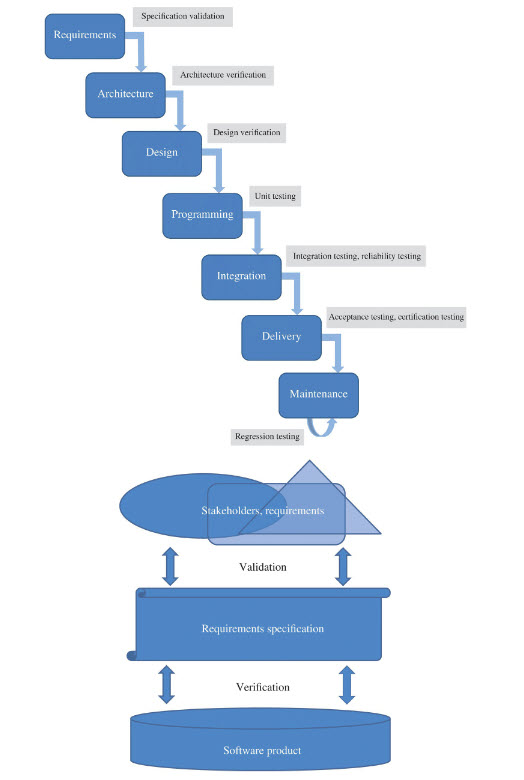
\includegraphics[]{figure31.jpg}

Figure 3.1 illustrates this lifecycle, and highlights the testing activities that take place therein. 

Each phase of this lifecycle concludes with a verification and validation step, intended to ensure that the deliverable that is produced in the phase is sufficiently trustworthy to serve as a launchpad for the next phase. 

Strictly speaking, validation ensures that the specification is valid (in the sense that it record all the valid requirements, and nothing but the valid requirements), whereas verification ensures that the product is correct with respect to the specification

\\
In theory, validation is used at the end of the requirements specification phase, and verification is used in all subsequent phases (see Fig. 3.2 for a summary illustration). 
\\
In practice, it is a good idea to maintain a healthy suspicion of the specification throughout the lifecycle, to test it at every opportunity (we will explore means to this end in subsequent chapters), and be prepared to adjust it as necessary.





